\ifdefined\included
\else
\setcounter{chapter}{8} %% Numéro du chapitre précédent ;)
\dominitoc
\faketableofcontents
\fi

\chapter{The director task: Assessing cognitive architectures}
\chaptermark{The director task}
\minitoc

The contribution presented in this chapter is excerpted from our work, submitted to the RO-MAN 2021 conference. This contribution closes this thesis and has been achieved in collaboration with other PhD students of the HRI teams. Guilhem Buisan was concerned about the task planning part. Amandine Mayima worked on the supervision component. Kathleen Belhassein has designed the presented task with us giving her psychologist point of view to create a task on which user studies could be performed. The engineer Yannick Riou worked on the motion planning component allowing us to develop a task where the robot acts on its environment. My concern about this task has been the integration of my previous contributions about Ontology and the REG. It has also been the opportunity to create an entire architecture extending the ones presented all along with this thesis and linked with the contributions of the team. Finally, I contribute to the Situation assessment component and on the Language understanding part.

The components related to my teammates will be briefly described to give an overview of the architecture. The newly introduced capabilities on which I work will be more detailed to explain the links I make between all my contributions, centred on the knowledge representation.

\section{Introduction}

Developing robotic architectures adapted to Human-Robot Interaction and thus able to carry out interactions in an acceptable way is still today a real challenge. The complexity comes, among other things, from the number of capabilities which the robot must be endowed with and therefore from the number of software components which must be integrated in a coherent manner. Such architectures should provide the robot with the capability to perceive its environment and its partners, to merge and interpret this perceptual information, to communicate about it, to plan tasks with its partner, to estimate the others' perspective and mental state, etc. Once developed, evaluating these architectures can be difficult because all these components grouped into a single system. The tasks we usually want the robot to handle must highlight a maximum of abilities, while still being simple enough to be reproduced by the community. Moreover, we should be able to conduct user studies with it to validate choices regarding naive users.

Since a long term goal of the robotic field is to see robots evolving in our daily life, many tasks and scenarios have been inspired by everyday activities. Even if these tasks offer a large variety of situation to ba handle since the human partner is not limited in its actions, they have the disadvantage of not highlighting some subtle abilities which are nevertheless necessary for good interaction.
The robot guide task \cite{satake_2015_should} in mall, museum, or airport, requires high communication skills to understand free queries (possibly involving chatting) and respond to them, whether to indicate a direction or to give advice. However, the perception needs can be limited due to the vast environments, as well as the perspective-taking needs due to the same perception of the environment by the robot and the human\footnote{For sure we can find some tricky cases where it could help but they do not reflect common situations.}. Finally, with such a task the human partner is not an actor of the task and just has to listen to the robot once their question is asked. Even if being in more constrained environments, bartender-like tasks~\cite{petrick_2012_social} have the same disadvantages. Indeed, the human is considered as a customer, and as such, the interaction with the robot is limited. The robot will never ask the human to help it for performing a task and their actions do not require coordination either full collaboration.

To involve the human partner in the task and requiring him to act with the robot, assembly-like tasks~\cite{tellex_2014_asking} can be used. Nevertheless, in most cases, the human acts as an assistant rather than as a partner as full collaboration can be challenging to perform. The robot thus elaborates a plan and performs the assemble, then asks for help when detecting errors during the execution (e.g., when it cannot reach some pieces). Here the task leads to unidirectional communication. Moreover, because in such a task both the robot and the human have equivalent knowledge about the environment, it can be hard to design situations where belief divergence appear and thus perspective-taking would be required.

Scaling down an everyday task to transform it into a toy task around a table can deduce the task complexity and allow easy reproducibility. Moreover, it allows making the robot and the human work in the vicinity of each other, with smaller robots for example. With the toy version of the assembly task presented in~\cite{brawer_2018_situated}, the human is more involved in the task. They ask the robot to take pieces and to hold them to help them assemble a chair. Even if the communication is unidirectional, we could imagine inverting the roles to test different abilities. Moreover, communication implies objects referring with the use of various visual features about the entities. Even if both agents have the same knowledge about the environment, the communication is grounded according to the current state of the world. In this task, no decision has to be made by the robot but once again, inverting the roles could open other challenges.

To focus studies around perspective-taking and belief management, the Sally and Anne scenario, coming from a psychology test, has been studied in robotic~\cite{milliez_2014_framework}. In this scenario, the robot is a spectator of a situation where two humans come and go from a room, and move an object from a box to another. Since a human is in the room when the other is acting, a belief divergence appears between the two humans and the robot has to understand it. While the task highlights the belief management, it is first limited regarding the perspective-taking since the human presence or not could be sufficient to estimate the humans beliefs\footnote{When both humans are in the room they have the same perception of the scene but have different beliefs about hidden objects. Perspective-taking would be required if the humans could lean over the boxes to check what is inside.}. Moreover, the humans do not act with the robot since it is just a spectator of the scene. In addition, no goal is formulated and the human neither interacts with one another. Finally, no communication is needed in the task. The scenario is thus focussed on the analyse of a situation.

In this chapter, we first propose a new psychology-inspired task that we think to be challenging for the Human-Robot Interaction community and rich enough to be extended: the Director Task. Inter alia, it requires perspective-taking, planning, knowledge representation with theory of mind, manipulation, communication, and decision-making. Then, we present the robotic cognitive architecture that we develop to perform the task in its nominal cases. Finally, on the basis of the presented task and what has been developed, we present a discussion about the possible future challenges and evaluations for the research community, with possible extensions of the task.

\section[From psychology to Human-Robot Interaction]{The Director Task: From psychology to Human-Robot Interaction}

In this section, we present the origins of the Director Task and the needs it aims to respond to regarding other tasks from the psychology. We then detail the setup we have designed in terms of objects characteristics and organisation in the environment. We end this section with our adaptation and the required abilities we have identified.

\subsection{The original task}

The Director Task has been mainly used in psychology researches as a test of the Theory-of-Mind usage in referential communication. This task originates from a referential communication game from~\cite{krauss_1977_social}. In this game, two participants are one in front of the other with an opaque panel between them. A speaker as to describe odd designs to a listener, either to number them for the adults or create a stack of cubes for the children. To refer to the odd figures, participants have to use images (e.g. "it looks like a plane").

This game was then adapted by Keysar et al.~\cite{keysar_2000_taking} and become the Director Task. It has been used to study the influence of mutual knowledge in language comprehension. In this task, two people are placed one in front of the other but instead of an opaque panel between them, they place a vertical grid composed of different cells and objects in some cells. The \textbf{director}, a participant or in most cases an accomplice, instructs the \textbf{receiver}, a participant, about objects to move in the grid. The receiver thus follows the director's instructions about objects to move. The particularity of the task is that some cells are hidden from the director meaning that the receiver, being on the other side of this grid, does not have the same perspective as the director. He thus knows the content of more cell than the director and consequently sees more objects. When the director instructs the receiver to move an object, for a successful performance, participants must take the perspective of the director to move the right one. Because the configuration evolves all along with the task, he has to update this estimated perspective all along with the interaction.

\begin{figure}[ht!]
\centering
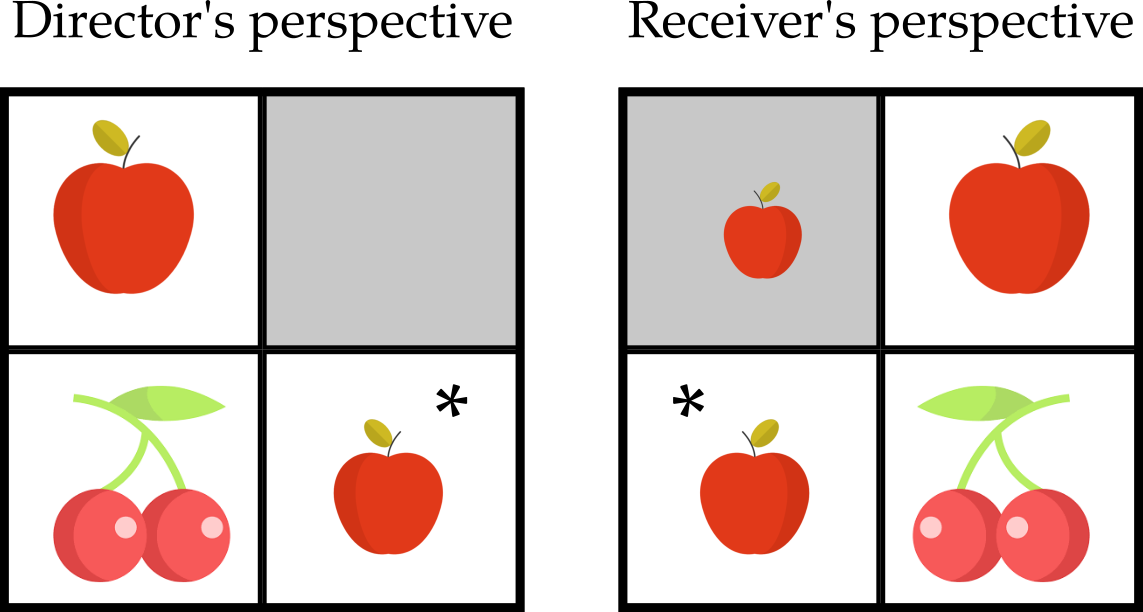
\includegraphics[scale=0.25]{figures/chapter9/dt_apple.png}
\caption{\label{fig:chap9_dt_apple} Sample display from the director's and the receiver's perspectives. The asterisk indicates the target object. Giving the sentence "the smallest apple" the receiver should find the good one even if he can see a smallest one in its perspective. }
\end{figure}

Taking the example of figure~\ref{fig:chap9_dt_apple}, if the director instructs the receiver to take the smallest apple, the target object in its perspective is the one marker with the symbol *. However, for receiver, in its perspective, the target object is not the smallest apple since the smallest one (called distractor) is only visible by the participant and not by the director. The participant then must understand the director's perspective to take the target apple and not the distractor. Some studies showed that for their first attempt, participants took the smallest apple from their own point of view and only after, the target one. These results were interpreted in~\cite{keysar_1994_illusory, keysar_1998_egocentric, keysar_2002_self, keysar_2003_limits} as the participants understanding language in an egocentric way. Some social cognition studies used a computer-version of the Director Task~\cite{dumontheil_2010_online} whose results are consistent with the ones mentioned previously, namely that participants do not use Theory-of-Mind inferences in language interpretation.

Although Theory-of-Mind and perspective-taking both require the attribution of mental states to others, some authors trend at distinguising Theory-of-Mind tasks and perspective-taking tasks as involving distinct although related mechanisms. In~\cite{santiesteban_2012_training}, they considered in their study that perspective-taking abilities were measured by the Director Task whereas Theory-of-Mind usage was investigated through another task called ``strange stories''~\cite{happe_1994_advanced}. This Theory-of-Mind task requires the attribution of mental states to a story protagonist, meaning to maintain an estimation of others' mental states. At the difference, the Director Task requires for adopting the perspective of the director in order to follow their instructions, meaning to use this knowledge in order to execute the task properly. 
In this way, the authors estimated that the Director Task requires a higher degree of self-other distinction by continuously isolating our own perspective from the director one, in order to use them to act. In addition to perspective-taking abilities, the Director Task makes use of executive functions~\cite{rubio_2017_director} (i.e. vary the processing of information according to current goals in an adaptive manner) and attentional resources~\cite{lin_2010_reflexively}.

To summaryse,the Director Task has been used to study referential communication, language comprehension, and perspective-taking abilities. However, to our knowledge, it has never been exploited in the context of a HRI although this task presents interesting challenges for this field. More than technical challenges, it provides a way to investigate the different cognitive and behavioral processes involved in such a cooperative Human-Robot task.

\subsection{The Director Task setup}

The material used in this task has been chosen to be easily acquired and can be hand-built. It is composed of blocks, compartments, and a storage area. Each element is equipped with AR-tags allowing the robot to perceive them without advanced perception algorithms.

\begin{figure}[ht!]
\centering
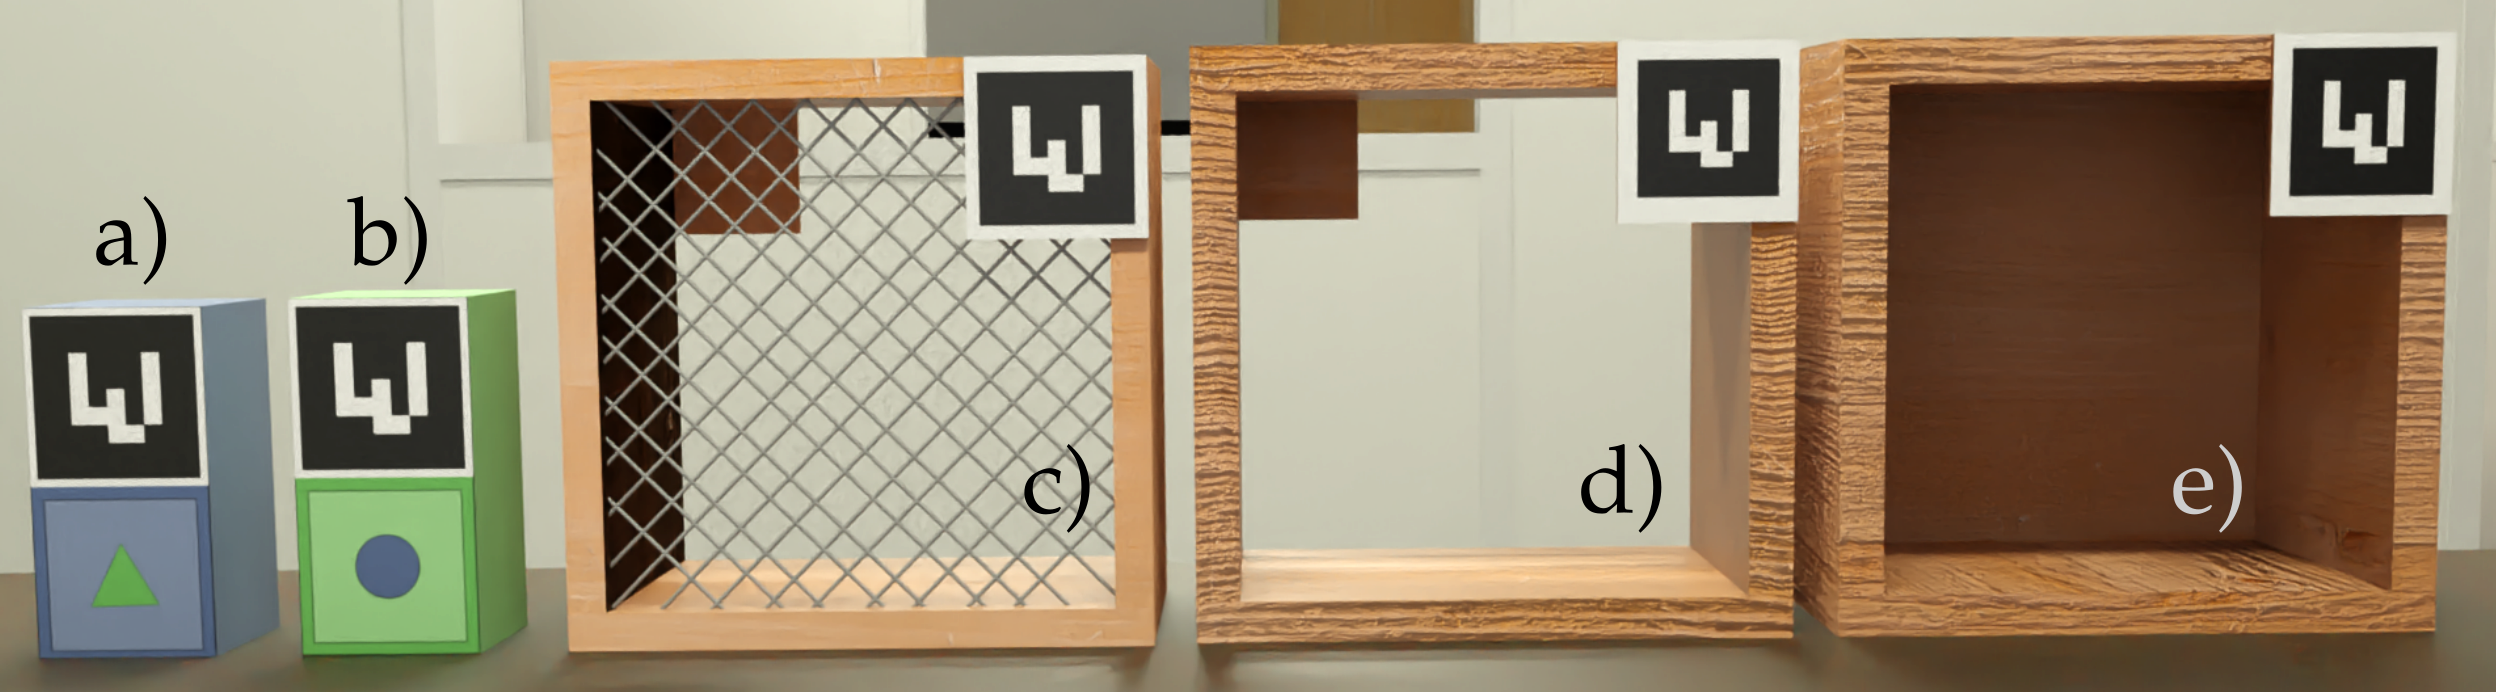
\includegraphics[width=\textwidth]{figures/chapter9/material.png}
\caption{\label{fig:chap9_material} Part of the material used for the Director Task. Each element is equipped with AR-tags allowing their detection by the robot. Each block has four visual characteristics: a main color, a border color, a geometric figure  and a figure color. }
\end{figure}

Three types of compartment exist and are illustrated on the right part of figure~\ref{fig:chap9_material}. The basic ones are open on two of their opposite sides (d). They allow both the receiver and director to see the content and to manipulate it. Others are open only on one of their sides (e). With such a compartment, only one of the participants can see and take what is inside. The other participant can neither know if a block is inside or not. The last compartment type (not used in the implemented version) has an open side and the opposite one equipped with a wire mesh (c). Because of the side with the wire mesh, both participants can see what is inside but only one of them can take it. Thanks to these three types, we will be able to vary the awareness of the blocks (e.g., a block is known to be present but not necessarily visible), the visibility of the blocks, and their reachability (e.g., a block can be visible but not reachable). While the original Director Task uses a vertical grid, we prefer here to use several compartments to create the grid. It allows more modularity to create different situations.

Where the tasks used in psychology use everyday objects, we rather choose blocks that can easily be manipulated by robots and on which we can fix tags for their detection (a-b on \ref{fig:chap9_material}). The blocks have a primary color covering them all. On two opposite faces, additional visual features are drawn. The top part of these faces is dedicated to the robot's perception with a unique AR-tag on each face\footnote{Since the tags are different on each side, the director can not refer to them as the receiver does not see the same ones}. The bottom part is the same on both faces and is dedicated to human perception. In addition to the primary color, three visual features are available by the human to distinguish them being: a colored border, a colored geometric figure (both the color and the figure can change making two features). Every visual feature (the colors and the forms) has exactly two variants. The colors are either blue or green and the figures are either a triangle or a circle. We can thus have 16 unique blocks.

The agents can use the four visual features to refer to a specific block and the complexity of the description depends on the used features. While the main color is directly related to a block, the other colors are respectively related to the border and the figure. In this way, for two blocks whose only difference is the color of one of these elements, the said element has to be referred to in order to refer to the divergent color. A description of a block involving all its four features would be ``the [color] block with the [color] border and the [color] [figure]''.

The figures and colors have been chosen in such a way to allow the emergence of ``coded words'' between the participant to identify a block. With a bit of imagination, some could refer to the left-most block (a) through the sentence ``the mountain in the sea'' or the other (b) by ``the puddle''.

\begin{figure}[ht!]
\centering
\includegraphics[scale=0.15]{figures/chapter9/positions.png}
\caption{\label{fig:chap9_positions} The Director Task setup with the robot and the human partner one in front of the other and a piece of furniture between them. Compartments are placed on top of the furniture and blocks are placed in the compartments. Next to the agent having the receiver role, here the human, a storage area is placed to drop the removed blocks. }
\end{figure}

Regarding the disposition, the compartments are stack on a piece of furniture to create a kind of grid. The blocks can be put in a compartment. As illustrated in figure~\ref{fig:chap9_positions}, the two agents are placed one in front of the other with the furniture and thus the compartment between them. Finally, one storage area, corresponding to the place where the receiver has to store the blocks, is delimited by a rectangle on a shelf next to the receiver. In the figure, the human would be the receiver as having the storage area on his right.

\subsection{The adapted task}

Now we see the Director Task setup and the available material, we present the rules we have adapted for HRI applications. First, the high-level goal of the task is known by both agents: to put a set of blocks away. The precise goal is given by the experimenter to the director, either the robot or the human. It corresponds to a subset of the blocks presents in the compartment that the receiver should remove from and put in the storage area. This choice to remove the objects instead of moving them in the grid engender an evolution of the situation over time. It thus requires a constant adaptation during the interaction. The goal can be given on a sheet of paper, a screen behind the receiver, or marks on the blocks on the director side. No block order is required in the formulation of the goal. The director is thus allowed to elaborate a strategy if needed.

As mentioned previously, the Director Task characteristics bring a number of interesting challenges for a collaborative robot to solve. Because this is a task with roles, one of the first challenges is to build a robotic architecture that gives the robot the ability to play both roles. Then, each role brings some specific problems to solve from a robotic point of view.

In order to enrich the task with perspective-taking issues, we adapted the task so that both the director and the receiver have to use perspective-taking. Since in the original task, the director knows he has a subset of the receiver's perspective, he can consider all the objects when communicating. Thus, only the receiver has to reason about the other's perspective, taking into account that some objects are not visible by the director. For HRI applications, we used the one side hidden compartments in a way to also have objects hidden from the receiver and visible by the director. Therefore, both roles have to perform perspective-taking, whether to give instructions or to understand them. On the illustration of figure~\ref{fig:chap9_setup}, the director (left image) can instruct the receiver to take the blue blocks as the other blue blocks in his perspective is hidden from the receiver. From the receiver point of view (right image), he can find the said block as the other blue block is hidden from the director.

\begin{figure}[ht!]
\centering
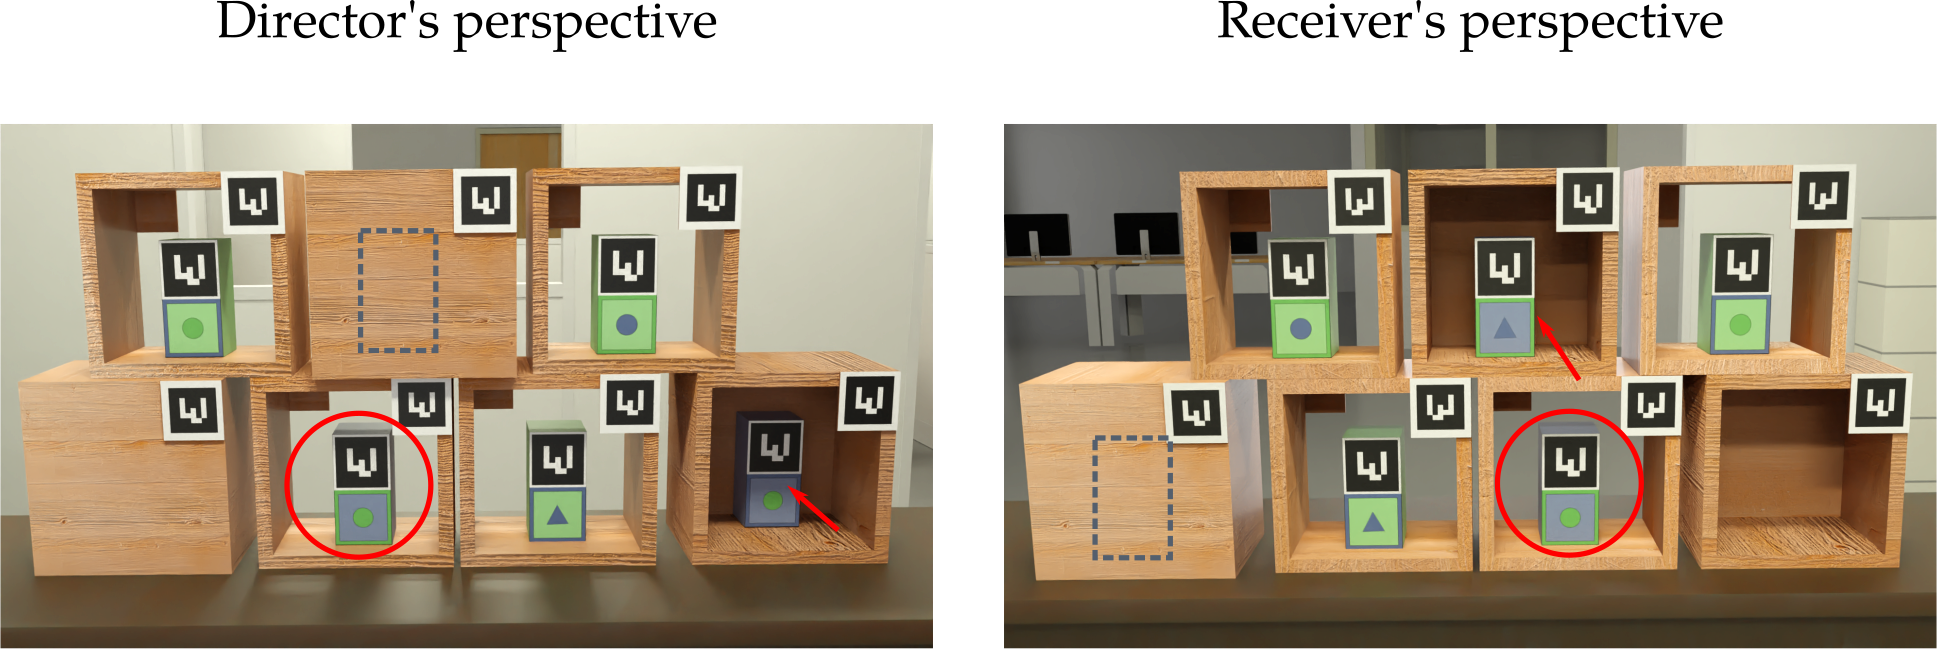
\includegraphics[width=\textwidth]{figures/chapter9/setup.png}
\caption{\label{fig:chap9_setup} A director task setup adapted to the HRI with the director's and receiver's perspectives. For the material, each element (blocks and compartment) is equipped with AR-tags allowing their detection by the robot. Each block has four visual characteristics: a main color, a border color, a geometric figure, and a figure color. Compartments can be hidden for the director or the receiver. For the director to designate the block marked with a red circle, estimating the receiver's perspective, he can refer to it by its main color (blue) because he estimates the other blue block is not visible by the receiver. For the receiver, by taking into account the director's perspective, he can understand the referred block as he estimates the other blue block to not be visible by the director.}
\end{figure}

To be able to study precise skills, such as verbal communication, perspective-taking, and adaptation, we defined a set of rules for both roles. First, the agents are not allowed to point to objects, either with their hand or gaze. They thus have to verbally describe the objects, focusing the task on verbal communication. However, to avoid too easy description of the kind ``the fully green block'', we remove the four uni-color variants\footnote{When we said too easy it is from the human point of view, generating and understanding such description can be challenging for a robot.}. In addition, to neither fall into simple referential communication task, participants are not allowed to use geometrical relations in the verbal communications. They cannot, for example, say ``the leftmost block'' or ``the block to the right of the green one''. In this way, they are limited to few visual features, with high ambiguity. Since a description of a block using its four visuals features can be hard for the human to process, we first expect the participants to minimize the complexity of their communication by referring to the blocks only using the features distinguishing them from other blocks. Moreover, we also expect the participant to take into account the other perspective allowing once again to minimize the complexity of the communication.

Over these elements, we can see that the task can easily be replicated and offer a controlled setup, making it a good task for human-robot user studies. Moreover, due to the number of involved processes and the number of situation that can be made, there are a lot of elements that can be analyzed and explored. Also, with the same setup, it is possible to perform human-human studies or human-robot studies which can be interesting to compare.

\subsection{Additional abilities}

More than being an easily reproducible scenario to perform user studies on human-robot interactions in a controlled environment, the Director Task allows demonstrating abilities of a robotic system. We detail here some additional abilities than the one the task has been designed for.

\paragraph{Planning} When a large number of blocks has to be taken in the task goal, it quickly becomes complicated to communicate about some of them as the director would have to add a lot of adjectives to be able to refer to one block. Therefore when the robot is the director, it becomes interesting to integrate the communication and the task planning. Indeed, depending on the order in which the blocks are designated, the complexity of instructions can decrease or increase. Then, the planner can return an optimal order in which the robot has to give the instructions to the human.

\paragraph{Contingencies handling} While performing the Director Task, errors can easily happen. Either because the director gives a wrong instruction or the receiver misunderstands the instruction and takes the wrong block. In both cases, it can be because of a wrong consideration of the other agent's perspective or simply inattention. Moreover, because some instructions might be right but hard to interpret by the receiver leading also to an error from them. Finally, errors can happen because of failure for the robotic system, as a failed action execution leading to a block to falls on the floor. A robot with a robust decision-making system will be able to analyze, try to determine their origin, and handle a number of these contingencies. For example, if the human takes the wrong block, the robot can react in different ways, either by asking the human to put it back if this block is not part of the goal, or saying nothing and re-planning if this block was among the ones to take. If errors happen repeatedly, the robot can also react differently than for a punctual error and maybe try to modify its behavior.

\paragraph{Communication} We saw that the task requires to put a focus on communications. The communication about an object can be more or less efficient, depending on the number of characteristics given about the object or the pertinence of these characteristics. Instructing for the blue block with a circle in figure~\ref{fig:chap9_setup}, the geometrical figure information is not mandatory. Thus, the robot needs to be able to give proper instructions but also to understand the human ones. Moreover, in complementarity with the error management, the robot can communicate to help to solve the detected contingency. Taking a situation (with the disposition of figure~\ref{fig:chap9_setup}) where the human as director instructs the robot with the green block with a circle. This instruction matching two blocks, the robot could say that it does not find the instructed block\footnote{It would be an easy solution for a stupid robot.}. A preferable reaction would be to help the human to refine the instruction and say "the one with a blue circle or a green circle ?".

\section[Architecture and knowledge link]{The cognitive architecture and the knowledge link}

In this section, we present the architecture developed to handle the Director Task in its nominal case for both roles. The architecture aims at being extending and already endow the robot with the abilities listed previously even if there are not mandatory to achieve the task. This architecture is the continuity of the one presented all along this thesis. It can also be see as a whole new instantiation of the deliberative architecture for Human-Robot Interaction presented in \cite{lemaignan_2017_artificial}. The seven identified modules are represented in figure~\ref{fig:chap9_architecture} with their respective communication links. In the rest of the section, we detail each module and how we have refined them in terms of functionality and linking. The modules already presented in this thesis will be briefly recall but not detailled in depth.

\begin{figure}[ht!]
\centering
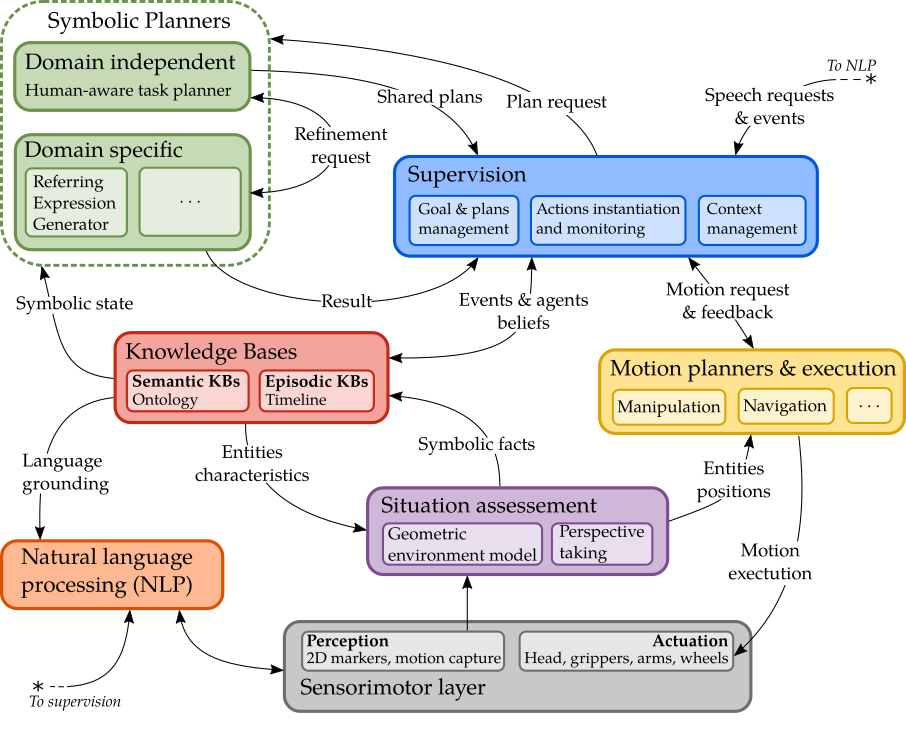
\includegraphics[width=\textwidth]{figures/chapter9/architecture.png}
\caption{\label{fig:chap9_architecture} An overview of the cognitive architecture developed to handle the Director Task. Each block does not necessarily represent one software component but rather an architectural module (in terms of the features it implements). The arrows represent the type of information exchanged between the modules. This architecture extends the ones presented all along with this thesis.}
\end{figure}

\improvement{Youtube link}
The architecture has been successfully implemented on a Pr2 robotic platform~\footnote{\url{https://cloud.laas.fr/index.php/s/kx6m67rt5n8bvky}} for both roles. The only emulated element is the human action recognition to trigger the next actions of the robot.

\subsection{Storing and reasoning on symbolic statements}

The knowledge representation is always a core component of cognitive architectures as organising knowledge allows the robot to better understand the environment it evolves in. Moreover, it is on the based of these knowledge that a robot can communicate with its human partner about the current state of the world and ground the partner's utterance regarding this world state.

Some architecture propagate knowledge all along their components~\cite{hawes_2007_balt}, each of them enriching knowledge at each stage before filling it to the nexts. Others have preferred to see their knowledge base as an active server, activating perception process when needed, depending the searched information~\cite{beetz_2018_know}. For our architecture, we staied on the principle of a central, server-based knowledge base. It is refined into two distinct sub-modules, the semantic knowledge base and the episodic one. The semantic part is in charge of representing the environment elements meaning, the objects' and agents' types, their applicable properties, the descriptions and parameters of the actions, a part of the language model with verbs or pronouns, and their names in natural language. Besides, we also use it to represent the current symbolic world-state (the computed facts) and thus the instantiation of the concepts in terms of physical (e.g., this particular block) or abstract (e.g., this particular action instance) entities. Among these instantiations, we have a part used for the interaction in itself, like the blocks' visual features, and others for the robot programming, like the objects' computer-aided design (CAD) models or tags ids. The episodic knowledge base aims at keeping a trace of the symbolic transitions of the world in the time. It is strongly linked to the semantic knowledge base as it allows to semantically interpret these transitions. 

The semantic knowledge base is still an ontology managed by the software Ontologenius. The episodic one is in the form of a timeline, managed by the software Mementar\footnote{\url{https://github.com/sarthou/mementar}}.

\subsection{Assessing the world: from geometry to symbolism}

The role of the geometrical Situation Assessment module is first to gather different perceptual information and build an internal geometric representation of the world, composed of objects and agents. From this world representation, the module runs reasoning processes to interpret it in terms of symbolic statements between the objects themselves and between the involved agents and the objects. Doing so, the module only builds the robot's representation. However, it does not necessarily reflect what the human partner believes about the world. This is the case with the occluded compartments of the task. If a block is present in a compartment occluded from the human perspective, this block is not visible and thus unknown to the human. Consequently. it should not exist in the human representation of the world. Here is the second role of the Situation Assessment module, estimating the human's perspective and building an estimation of their world representation. It is the first step allowing to implement the theory of mind principles \cite{baron_1985_does}.

To implement this module, we have chosen the Underworld framework~\cite{lemaignan_2018_underworlds}. Its advantage is to not be monolithic\footnote{It can however be a disadvantage in terms of performance but for research purpose, it allows more flexibility.}. It works on the principle of a set of worlds, each working at a different granularity and providing specific features, links to create a so-called cascading structure. In the idea, it can be compared to a perception pipeline like~\cite{beetz_2015_robosherlock}. It allows easy reuse of existing modules and makes the core reasoning capabilities independent of the used perception modalities. Where we choose to use tags for objects detection, we could easily pass to machine learning approaches. In the same way, we could use it with simulations or Virtual Reality systems.

The four worlds we create for the Director Task and their connexion are represented in figure~\ref{fig:chap9_uwds}. At the top (a), we have the perception modalities. For the objects we use AR-tags~\cite{fiala_2005_artag}. For humans, we use a motion capture (mocap) system with helmets equipped with reflectors. For now, only the head is tracked. From each perception input, we create a dedicated world. In these worlds, we can filter the perception data depending on the used system. For the mocap, the data is clean enough. For the AR-tags we apply first a motion filter to discard data acquired when the robot moves. In addition, we apply a field of view (FOV) filter to discard data from the border of the camera because of distortions giving wrong positions even with camera calibration. To know to which object correspond a given tag unique identifiers (UID), the worlds have access to the ontology and can query it to get the UID related to. In the same principle, they can get the objects CAD model. As the output of these worlds, we ensure to have stable data with UID related to the knowledge base.

\begin{figure}[ht!]
\centering
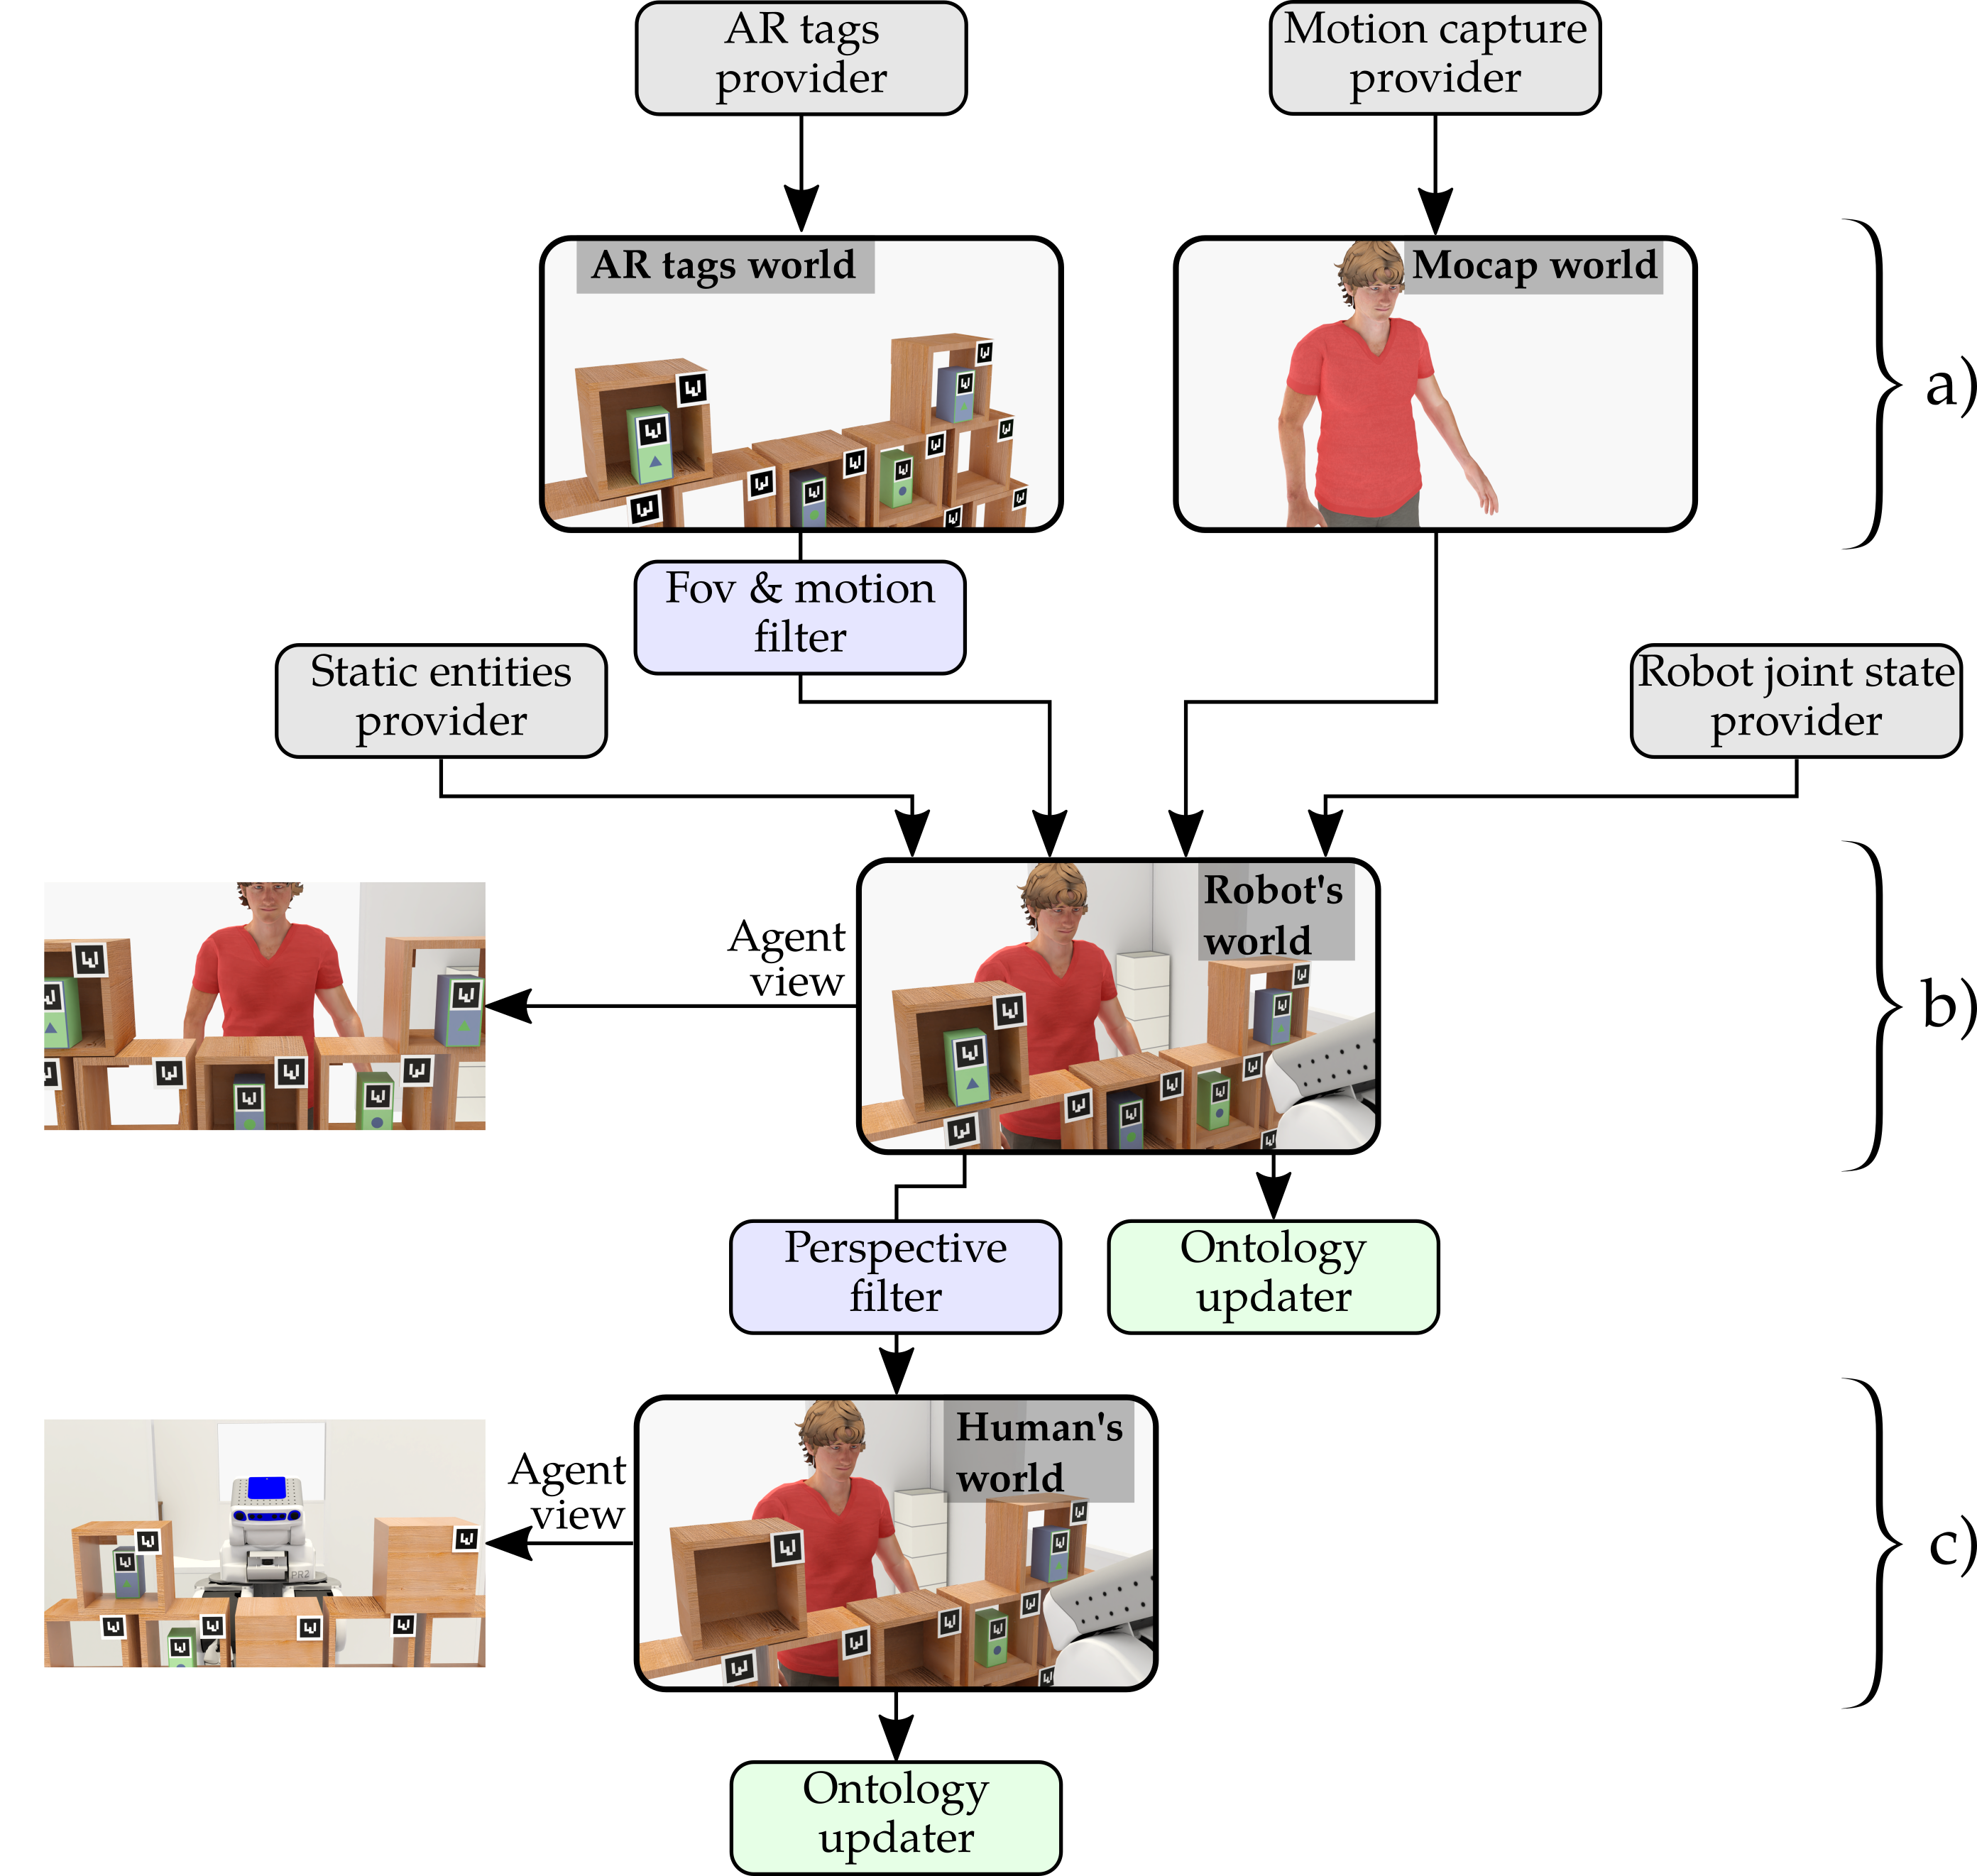
\includegraphics[width=\textwidth]{figures/chapter9/uwds/uwds.png}
\caption{\label{fig:chap9_uwds} The world cascading structure of the geometrical situation assessment system. The two worlds at the top (a) are build from the perception systems and filtered. The world of the middle (b) merges the different perception information and computes symbolic facts on it. The world at the bottom (c) is the estimation of the human world representation and is computed from perspective-taking in the robot's world. Like for the world of the middle, symbolic facts are computed and sent to the semantic knowledge base.}
\end{figure}


The world of the middle (b) is the robot's world representation. Information from the perception worlds is merged along with the static elements, like the building walls, and the robot model. From this world, additional perception reasoning processes are applied for the objects that are no more visible in the way of~\cite{milliez_2014_framework}. If an entity is no more perceived in one of the previous worlds, we first test if it should be in the robot's FOV. If so, the robot should see it. To get an explanation of this absence, we test if another entity could hide it. If not, the object is removed from the world representation. Otherwise, we keep it as we have found an explanation.
Once the entities stabilised, geometric reasoners are applied to them to extract symbolic facts. In the current version of the system, the computed facts are \textit{isOnTopOf}, for an object on top of another with a direct contact, \textit{isInside}, for a block in a compartment, \textit{isVisibleBy}, assessing if an agent could see the object or not from his position, and \textit{isReachableBy}, assessing if an object can be taken by an agent. All these facts are sent to the robot's semantic knowledge base, where reasoners will deduce further facts. For example, if a block is in a compartment, thanks to inverse property \textit{hasInside} the fact that the compartment has the block inside is computed. In the same way, if this compartment is on top of the table, the block inside is computed to be above the table (\textit{isAbove)} thanks to chain axiom.

While the previous world corresponds to the robot's representation, the human partner can have the same because of the occluded compartments. The world below (c) thus aims at estimating the representation of the world from the partner's perspective. From the robot's world, we compute a segmentation image from the human point of view and use it as a filtered perception world. This allows us to instantiate the same world management process we used for the robot but this time for the human. In this way, we emulate their perception capability and geometric reasoning process. Symbolic facts are thus computed and sent to the human's semantic knowledge base. In the world of the bottom on figure~\ref{fig:chap9_uwds}, we can see that the two blocks in the occluded compartments are not present in the human world. Here we make explicit the difference between an object that is unknown and an object that is known but not visible. We could have an interaction where the human goes to see the robot side and the robot would consequently estimate the blocks in the occluded compartments as known to the human but not visible.

\subsection{Planning with symbolic facts}

The symbolic planners are divided into two categories: the domain-independent, planning high-level tasks, and the domain-dependant, specialized in solving precise problems. For the Director Task, the only domain-specific planner used is the Referring Expression Generator presented all along with this thesis. More precisely, we integrate the algorithm presented in chapter~\ref{chap:chap7}.

Where we previously used HATP~\cite{lallement_2014_hatp} as task planner, for this task we used its next-generation presented in~\cite{buisan_2021_human}. In the same way, it aims at taking into account the human's contribution to planning how to perform a high-level task. To do so, it can generate a shared plan in which parts of the task are assigned to the human partner, depending on some criteria. However, the robot's partner is not an agent that the planner can directly control. Indeed, it must sometimes communicate about the plan to inform the human about their next actions. The new planner rather trends at emulating the human decision, action, and reaction processes to generate a shared plan. For the Director Task, emulating the human reaction to a given instruction enables the comparison between multiple blocks order, the communication of higher-level instructions to the human and the balance between multiple communication modalities.

The REG planner has been successfully integrated with the new planner allowing it to estimate the cost and the feasibility of referring communication at task planning. The initial world state is fetched from the ontology leading to a uniformity of the knowledge among the architecture.

\subsection{Managing the interaction}

The supervision component aims at managing the overall interaction. In this architecture, we use JAHRVIS (Joint Action-based Human-aware supeRVISor) which constitutes the decisional kernel of this cognitive architecture. Like its predecessors, SHARY~\cite{clodic_2009_shary} and its extensions~\cite{fiore_2016_planning, devin_2016_implemented}, it is designed for a human-aware robot. It has to not only handle the robot's action execution but also estimating the human mental state, monitoring his actions, and communicate with him. To handle these features, several processes are needed:

\paragraph{Interaction sessions management:} It manage an interaction session that is first refined into tasks, themselves refine into action with the use of the task planner. Moreover, it is in charge of the greetings happening at the beginning of an interaction, the goodbyes at the end, and all events and exchanges happening outside tasks (e.g., conversation, goal negotiation) or during a task but not related to it like a human doing a parallel task on its own.

\paragraph{Communication management:} Communications are categorized in JAHRVIS either to: give information updating the receiver beliefs; ask a question to update the emitter belief; ask the other agent to perform an action; discuss with dialogue not related to a task or a goal/plan negotiation. 

\paragraph{Human management:} As the supervision manage shared plans, it has to make sure the human follows them. Moreover, even if some communications are plans, it also has to make sure that the human has all the knowledge they need for what they have to perform and if not, it hence acts or communicates through the other processes. To do so, it monitors the human beliefs about the ongoing task and plan.

\paragraph{Task management} Even if the human has also the necessary information about the plan, contingency can happen. The supervision can react and perform a repair thanks to action or communication.

\paragraph{Quality of Interaction management} Even if a task is achieved, it could be done more or less efficiently and smoothly. All along an interaction session and a task, the supervision thus estimates in real-time the Quality of Interaction (QoI)~\cite{mayima_2020_toward}. It measures the human engagement and the effectiveness of collaborative task performance. This information can then be used by the decision-making process to tune dynamically others processes such as the cost of properties for the REG.

\subsection{Speaking and understanding}

The Natural Language Generation is made of two parts, a static for actions verbs and communications to signify a lack of understanding and a dynamic part for the referring expressions. In the same way, we already done, the content is determined by the REG and the linguistic realisation is done on the basis of concepts' labels in the ontology and a simple grammar model to know in which order the adjectives have to be depending on the language.

Natural Language Understanding is more difficult due to the variety of way the same information can be communicated. Moreover, in the same communication, we have different information. In the Director Task, we have the action to perform and the object on which the action has to be performed. First, we use the Google Speech To Text (STT) API to pass from an audio stream to a string of characters. Even if such technology is now well mastered, mistakes still appear in the transcription\footnote{And this, even more, depending on our English accent and the quality of the microphone used}. On the string, we perform a first analysis trying to match words and group of words with labels of the ontology. We used sliding windows limited on the length and the fuzzy match technique available with ontologenius. To cover a maximum of possibility, several actions verbs are described as well as synonyms for the concepts. We also tried to have a good hierarchy in the ontology types for the robot to better catch the concepts depending on the abstraction level used by the human. To refer to the blocks, some only use the terms "object" as they are the only ones involved in the task. At the end of this analysis, we have a list of concepts. Depending on the number of uncaught words, we can already know if the comprehension is poor or not. On the concept list, we first extract the action verb to know the instructed action (e.g. take, place, remove). The rest of the sentence is analysed thanks to the inverse grammar model for one part but also thanks to the properties ranges and domains. When we said "the red apple", we do not have any word representing the used property\footnote{It is often the case of the attributes where relations between entities are more explicit.}. With the analyse of the usable properties linking color to an apple (and thus to a vegetable and so on), we are able to find the corresponding property. The result of this analyse is a \sparql{} query in the same way such query is used for the NLU. Depending on the number of concepts successfully linked we can estimate the comprehension quality. The \sparql{} describing the entity to act on is then merged with the context of the task and sent to the onology to find the target entity. In our case, the context would be the same as for the generation meaning that we are speaking about an object being above the table of interaction.

In the case the human gives an accurate description, we should have only one match for the target entity. However, we can not consider that the human will never do a mistake or that the robot will fully understand the instruction. In this case, we run a REG on all the ambiguous entities. The context of these generations is the \sparql{} query coming from the understanding process. If we know that we are already speaking of a green block, we do not have to recall it. We fall back into Natural Language Generation and generate sentence like "do you mean the block with a circle or a triangle ?". When the human response, we use again the \sparql{} query coming from the first utterance and merge it with the newly understood.

For the Natural Language Understanding part, we could use machine learning approaches based on sequence-to-sequence (seq2seq) models like~\cite{panchbhai_2020_exploring}. However, doing so we duplicate the knowledge already existing in the ontology to put them in a neural network. Unless creating a standard of concept identifier, such model should be trained for each used knowledge base in order to be compatible with it and use the same symbols. Having different symbols would lead to failure, having more symbols in the trained model would lead to failure (queries that could not match), and having fewer symbols in the trained model would lead to a lack of comprehension. Moreover, in addition, to create the ontology, we would have to create the corresponding training dataset that is a huge amount of work even if artificially augmented dataset creation techniques exist.

Even if our method can be seen has been ha-doc, we ensure uniformity of the knowledge among the architecture. Moreover, it can be easily extended and even dynamically extended during an interaction.

\section{Open challenges for the community}

So far, we have described the main abilities a robot has to be endowed with to perform the Director Task. Then, we have proposed a cognitive robot architecture handling the Director Task in its simplest form, both for the director and receiver roles. However, we have only tackled the normals cases that the task offers. In this section, we now present some open challenges that we have identified around the task. In addition, since we see that the environment of the task can be controlled, we also propose some user studies to investigate the ways of sharing information.

\subsection{Challenges to take up}

The components or abilities related to each challenge are reported in the following table. The list of challenges is not exhaustive. Moreover, even if some challenges have already been mentioned among the presentation of the components, they are here reported as requiring finer and more generic management.

\begin{center}
 \begin{tabular}{||l | l ||} 
 \hline
 Challenged abilities / components & Challenges \\ [0.5ex]
 \hline\hline
 Perspective-taking & \ref{chal:cont_analysis}  \\ 
 \hline
 Communication & \ref{chal:change}, \ref{chal:understand}, \ref{chal:words}\\
 \hline
 Task planning & \ref{chal:cont_errors}, \ref{chal:cont_not_errors}, \ref{chal:change} \\
 \hline
 Reference generation & \ref{chal:change}, \ref{chal:spatial_ref}, \ref{chal:multi} \\
 \hline
 Contingencies handling & \ref{chal:cont_analysis}, \ref{chal:cont_errors}, \ref{chal:cont_not_errors}, \ref{chal:change} \\ [1ex]
 \hline
\end{tabular}
\end{center}

\begin{enumerate}

\item \textbf{Finer contingency analysis:} In this task, failures can easily arise due to the high ambiguity between the blocks and the difference of perspective. Such failures have to be handle by the robot and to do so their origin have to be understood to react to them in an appropriate meaner. In the case the human as the receiver does not take the instructed block, the failure can have different origins. First, it could come from a perspective not taken into account. However, this lack of perspective-taking can be assigned either to the director or the receiver. Another origin can be a description not clear enough or correct but too complex. Finally, it can just be an error of inattention. Each of these origins has to be handle in a different way. \label{chal:cont_analysis}

\item \textbf{Handling contingencies as errors:} When the receiver takes another block than the one instructed, has to fix the error through communication and negotiation. First, the wrong block has to be put back in its original compartment. Then, the robot has to adapt its original instruction to make it clearer and improve the chances to have the receiver taking the right one.\label{chal:cont_errors}

\item \textbf{Not handling contingencies as errors:} When the receiver takes the wrong block, even if it is the instructed one, it can however be part of the goal. In this case, the robot not necessarily has to repair the plan, asking the human to put it back as no order is required for the task. It can thus re-plan or re-instruct the human for the same block without further information. It may also mention to the receiver for the mistake and explain that it does not matter because this one is also part of the goal. Rather than re-planning, the robot could use a conditional plan, anticipating possible confusions, and adapt according to the human's actions.\label{chal:cont_not_errors}

\item \textbf{Adapting to recurrent failures:} In case of recurrent failures by the partner or degradation of the Quality of interaction with numbers of latencies, the robot could try to analyse the origin of the problems and determine if a common point exists. If so, it can adapt itself to increase the QoI and reduce the failures. For example, if the partner is found to have difficulties with certain visual features, the robot can react through properties' cost adaptation. If the partner still consider the removed blocks, it can react through communication context adaptation.\label{chal:change}

\item \textbf{Allowing spatial references:} As explained in section in the origins of the task, the Director Task is originally a task to test referential communication. Even if the present version asks the participants to not use spatial reference, this rule could be relaxed to study perspective-corrected spatial Referring Expression Generation.\label{chal:spatial_ref}

\item \textbf{Understanding the human instructions:} In the current implemented version, the robot can only understand a limited vocabulary and restricted to the context of the task. In this way, the robot only understands descriptions of blocks. In a more natural interaction, humans could use a richer vocabulary, give a single instruction in multiple steps, or have communications not directly linked to the task. During tests for designing the task, it was common to have instructions like ``take the block with a ... triangle. No, rather the one with a green border''. Such complex communications where the director corrects his explanations should have to be managed by the robot.\label{chal:understand}

\item \textbf{Introducing code words:} As presented through the design of the used material, the visual features on the blocks have been chosen in a way to allow the visualisation of landscapes on them, with a little imagination. Considering multiple tasks with the same robot and human, alternating the roles if needed, the introduction of coded words could be interesting to reduce the communication complexity and thus the overall efficiency. The robot could thus try to negotiate some coded words. Once introduced, it would also have to remember them and understand them as being part of a description. \label{chal:words}

\item \textbf{Communicating about multiple blocks:} With the currently implemented system, the director only instruct one block at a time. It can either be through a reference matching all of them, like ``Take all the blocks with a triangle on them'', or multiple descriptions in a raw. The latter method could bring different kinds of communications such as ``I do not remember the instruction for the last block'' when the human is the receiver. For the first method, when the robot is the receiver, it would also be a different kind of instructions to interpret.\label{chal:multi}
\end{enumerate}

\subsection{User studies to perform}

Some robot behaviours, mainly about the referring expression generation, have been designed with regard to the current literature. However, the Director Task could be used to refine them thanks to user studies. More than providing a controlled task and environment, this task has the advantage to hide the real goal of the study. From the participant point of view, the goal is to remove blocks from compartments. The goal of the study can be focused on other aspects and could help the community in the design of architectures applied to more realistic scenarios.

Currently, the references to the blocks are made in such a way as to minimize the number of visual features used while staying discriminative. Such implementation fit Grice's Maxim of Quantity \cite{grice_1975_logic}. However, due to all the cognitive mechanisms to use in this task (e.g., perspective-taking) and the high ambiguity among the blocks, evaluating such behaviour compared to a full explanation could be interesting. Indeed, giving a reference with more information than needed would ensure to not match blocks being only visible by the receiver, which could help them to select the right block. In a way, it could allow to not use perspective-taking at the cost of complex communications.

During the material presentation, we have introduced a special compartment equipped with a wire mesh. Because a block in such a compartment is visible from the receiver but not accessible, referring to a block matching also this one could disturb the receiver. We could expect such a situation to require a higher cognitive load to determine the right block to take. Such behavior could also be interesting to evaluate as even if the human receiver is able to take the right block it could also decrease the Quality of Interaction. In the same way, a block previously visible by the receiver and that the director moves in a hidden compartment could disturb the receiver to interpret a description.
